\section{Theoretical Analysis}
\label{sec-theory}

In this section, we present an analysis of the reachback scheme for
two oscillators. Our analysis follows that of Mirollo and
Strogatz. The ideas and mathematical constructs used are similar,
though they differ in important ways that require slightly more
complex analysis.

Each oscillator is characterized by a state variable $s$ that evolves
according to $s=f(\phi)$ where $f$ is the firing function and $\phi$
is a phase variable representing where the oscillator is in its
cycle. For example, if an oscillator has finished 3/4 of its cycle,
then $\phi=3/4$. Thus $\phi\in[0,1]$ and $d\phi/dt=1/T$ where $T$ is
the period of the oscillator's cycle. We assume that the function $f$
is monotonic, increasing, and concave down. For our purposes, we
choose $f(\phi)=\ln(\phi)$.

Now consider two oscillators A and B governed by $f$. They can be
visualized as two points moving along the fixed curve $s=f(\phi)$ at a
constant horizontal velocity $1/T$, as shown in Figure
\ref{fig:theory2}. When A reaches $\phi=1$ it will fire, and B will
record the phase at which it hears A's firing. In the RFA scheme,
unlike the M\&S model, B will \emph{not} jump immediately upon hearing
A's fire; instead, B will record the time and then execute the
appropriate jump after its next firing. The jump is defined as
$\Delta(\phi)=g(f(\phi)+\epsilon)-\phi$, where $g=f^{-1}$ and
$\epsilon \ll 1$. For example, if B records $\phi_1$ as the time A
fired, when B reaches $\phi=1$ it will fire and then jump forward to
$\phi=\Delta(\phi_1)$. In the the RFA scheme, $f(\phi) = \ln(\phi)$
(and thus $g(\phi)=e^{\phi}$), therefore
$\Delta(\phi)=(e^{\epsilon}-1)\phi$. The question is whether the RFA
scheme leads to synchrony.

\begin{figure}[t]
\begin{center}
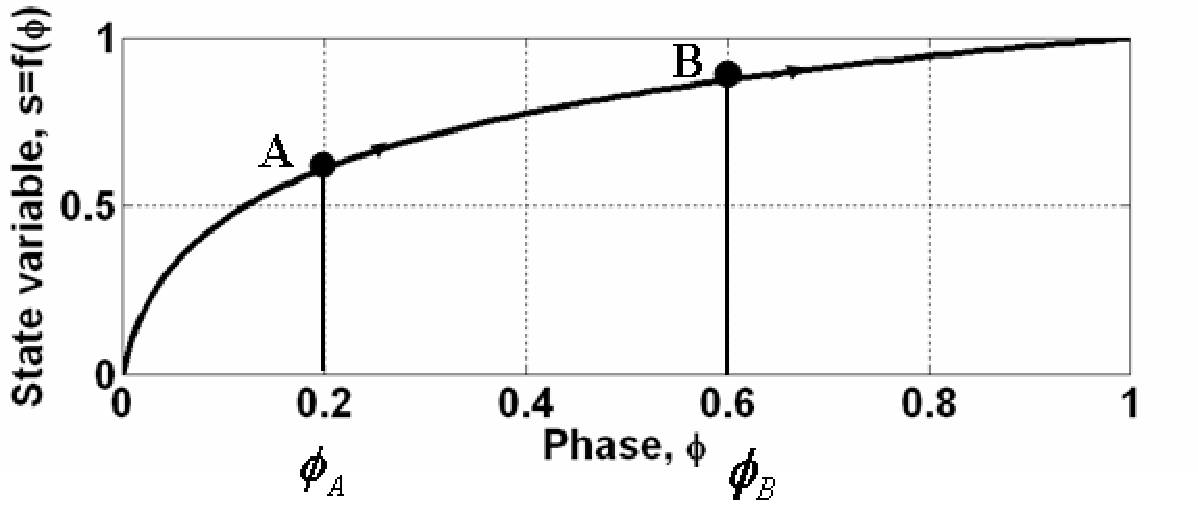
\includegraphics[width=1.0\hsize]{./figures/theory-2oscillators.pdf}
\end{center}
\caption{Two nodes A and B moving along $s=f(\phi)$}
\label{fig:theory2}
\end{figure}

\newtheorem{theorem}{Theorem}
\begin{theorem}
Two oscillators A and B, governed by RFA dynamics, will be driven to
synchrony irrespective of their initial phases.
\end{theorem}

{\bf Proof.} Consider two oscillators A and B. Consider the moment
after A has fired and jumped. In the instant after the jump, let
$\vec{\phi} = (\phi_A,\phi_B)$ denote the phases of oscillators A and
B, respectively. The {\em return map} $R(\vec{\phi})$ is defined to be
the phases of A and B immediately after the \emph{next} firing of A
(which is necessarily \emph{after} the next firing of B since A cannot
jump past B\footnote{If A fires and then jumps to $\phi_A$, then
$\phi_A \leq \phi_B$ for the following reason: If the phase of B is
$\phi_B$ when A reaches $\phi=1$, then A must have observed $B$ fire
at $\phi_x \geq 1 - \phi_B$ (since B would have fired and then taken a
positive jump). After firing A takes a jump of
$\phi_A=\Delta(\phi_x)$. $\Delta(x)$ is always $\leq 1-x$ because it
is truncated to never cause a jump past the end of the
cycle. Therefore $\phi_A \leq 1-\phi_x \leq \phi_B$.})

We now calculate the return map $R(\vec{\phi})$. Without loss of
generality assume $\phi_A < \phi_B$. Since A has just fired, B records
A's firing time as $\phi_B$. Both oscillators move forward in their
cycles until B fires. After B fires, according to our algorithm, B
jumps to phase $\Delta(\phi_B)$. In the meanwhile, A has moved forward
a distance $1-\phi_B$, reaching phase $\phi_A+1-\phi_B$, and recording
this as B's last firing time. After A's next firing, it jumps to
$\Delta(\phi_A+1-\phi_B)$, and B is at
$\Delta(\phi_B)+1-(\phi_A+1-\phi_B) =
\Delta(\phi_B)+\phi_B-\phi_A$. Substitution of the expression for
$\Delta(\phi)$ and algebraic simplification yields:

\begin{equation}\label{dynamics}
\vec{\phi}_{n+1}=R(\vec{\phi}_n)=M\vec{\phi}_n+\vec{b}
\end{equation}

Here $n$ denotes the cycle number. The vector $\vec{b}$ is defined as
  $(e^\epsilon-1,0)$, and the matrix $M$ is defined as


\begin{equation}\label{ADefn}
M=
\begin{bmatrix}
  e^\epsilon-1 & -(e^\epsilon-1) \\
  -1 & e^\epsilon \\
\end{bmatrix}
\end{equation}

%% \begin{equation}\label{bDefn}
%% \vec{b}=
%% \begin{bmatrix}
%%   e^\epsilon-1 \\
%%   0 \\
%% \end{bmatrix}
%% \end{equation}

Hence the algorithm can be described as a
linear dynamical system in $\vec{\phi}$, where $\vec{\phi} \in
[0,1] \times [0, 1]$. The unique fixed point of this dynamical
system is easily shown to be:

\begin{equation}\label{fixedPtDefn}
\vec{\phi}^*=
\begin{bmatrix}
  0 \\
  \frac{1}{2} \\
\end{bmatrix}
\end{equation}

\begin{figure}[t]
\begin{center}
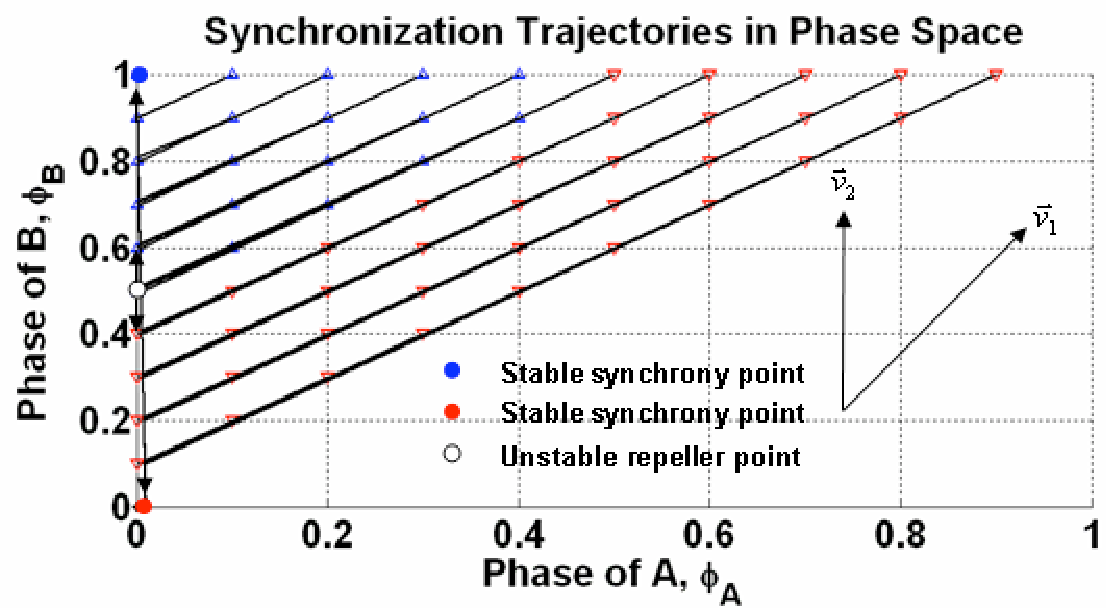
\includegraphics[width=1.0\hsize]{./figures/theory-trajectory.pdf}
\end{center}
\caption{Trajectory of the oscillator phases}
\label{fig:theory1}
\end{figure}

At $\vec{\phi}^*$ both A and B would be exactly half a cycle apart. We
now show that $\vec{\phi}^*$ is unstable (i.e.. a "repeller") such that
the phases gets pushed to either (0,0) or (1,1) where the dynamics no
longer change. Introducing the change of variables
$\vec{\varphi}_n=\vec{\phi}_n-\vec{\phi}^* $ we can rewrite
(\ref{dynamics}) as

\begin{equation}\label{shiftEqn}
    \vec{\varphi}_{n+1}=M\vec{\varphi}_n
\end{equation}

By the eigendecomposition theorem, we can decompose $M$ as
$M=V\Lambda V^{-1}$, where $V$ is the matrix of composed
eigenvectors and $\Lambda$ is a diagonal matrix containing the
eigenvalues of $M$. To leading non-vanishing order in $\epsilon$,
the eigenvalues (in $\Lambda$) are $\lambda_1=\epsilon^2$ and
$\lambda_2=(1+\epsilon)$, and the principal eigendirections (the
rows of $V^{-1}$) are $\bar{v}_1=(1,1)$ and
$\bar{v}_2=(0,\epsilon)$. The decomposition allows us to rewrite
(\ref{shiftEqn}) as

\begin{equation}\label{changeOfBasisEqn}
    \vec{\theta}_{n+1}=\Lambda\vec{\theta}_{n}
\end{equation}

where $\vec{\theta}_{n}=V^{-1}\vec{\varphi}_n$ is a change-of-basis
transformation that maps all vectors into a new coordinate system
spanned by the basis $\mathcal{B}=\{\bar{v}_1, \bar{v}_2\}$. Equation
(\ref{changeOfBasisEqn}) shows us that the evolution of the system is
most simply described in terms of $\mathcal{B}$. The system's
evolution along the directions $\bar{v}_1$ and $\bar{v}_2$ is
illustrated in Figure \ref{fig:theory1}. First, all trajectories
rapidly approach the $\phi_A=0$ axis along the vector
$\bar{v}_1=(1,1)$ since $\lambda_1=\epsilon^2 \ll 1$. Upon reaching
the axis, trajectories are repelled away from $\vec{\phi}^*=(0, 1/2)$,
along the direction $\bar{v}_2=(0,\epsilon)$, since $\lambda_2 >
1$. If a trajectory approaches the axis from below $\vec{\phi}^*$, it
will slide down the axis to the state of synchrony
$\vec{\phi}=(0,0)$. Otherwise, it will climb up to $\vec{\phi}=(0,1)$,
another state of synchrony. Thus $\phi^*$ is a repeller and the
oscillators are driven to synchrony, irrespective of initial
phases. QED\\

{\bf Rate of synchronization.} How quickly the system
synchronizes depends on how fast it moves in the $\bar{v}_2$ direction
away from $\vec{\phi}^*$ before it reaches a state of synchrony. We
can estimate the time to synchronization, starting from
$\vec{\phi}^{(0)}=(\phi_A^{(0)}, \phi_B^{(0)})$. Given such an initial
state, the system's trajectory will intersect the $\phi_A=0$ axis at
approximately $\delta=\phi_B^{(0)}-\phi_A^{(0)}$. The distance from
the fixed point grows exponentially fast with eigenvalue
$\lambda_2=(1+\epsilon)$ in the $\bar{v}_2$ direction. Let $k$ denote
the number of iterations required. Solving $\lambda_2^k
(\delta-\frac{1}{2}) = \frac{1}{2}$ yields

\begin{equation}\label{rateOfSync}
    k = \frac{1}{\ln(1+\epsilon)} \ln(\frac{1}{2\delta-1}) \approx
    \frac{1}{\epsilon} \ln(\frac{1}{2\delta-1})
\end{equation}

Thus, \emph{the time to synchrony is inversely proportional to
$\epsilon$}.

\newpage

Note that these proofs are very similar to the two oscillator case for
Mirollo and Strogatz, and most likely can be extended to $n$
nodes. However extending these results to multi-hop topologies
requires considerably more sophisticated analysis
\cite{lucarelli04}. Instead we evaluate the algorithm in simulation
for different $n$ and network topologies.



